\chapter{Analisis}
\label{chap:analisis}

Privasi yang perlu dijaga antara lain mengenai identitas seseorang atau hal yang dapat dikaitkan terhadap identitas seseorang. Pada data yang digunakan untuk penambangan data sangat banyak sekali data privasi tersebut sehingga perlu adanya cara untuk menjaga privasi tersebut. Metode randomisasi dapat digunakan untuk menghilangkan privasi pada data tetapi masih dapat dilakukan penambangan data. Metode yang dipilih untuk diimplementasikan adalah teknik \textit{Random Rotation Perturbation} dan \textit{Random Projection Perturbation}. Tetapi ada kekurangan pada kedua teknik tersebut. kekurangan tersebut adalah nilai setiap fitur yang ada pada data harus bersifat numerik dan kedua teknik tersebut hanya menjaga jarak Euclidean sehingga hanya teknik penambangan data yang bergantung pada jarak Euclidean saja yang dapat digunakan.

\section{\textit{Random Rotation Perturbation}}
\label{subsec:rrp}

Seperti yang telah dijelaskan di bab~\ref{chap:teori}, ide dari teknik \textit{Random Rotation Perturbation} adalah merotasi seluruh data yang direpresentasikan sebagai titik pada bidang Euclidean sehingga jarak antara titik-titik yang ada tidak berubah walaupun nilai tiap titik berubah secara drastis. Berikut akan ditunjukkan algoritma dan studi kasus yang telah dilakukan pada teknik \textit{Random Rotation Perturbation}.

\subsection{Algoritma}
\label{subsec:algo-rotation}

Algoritma \textit{Random Rotation Perturbation} mempunyai beberapa langkah yaitu sebagai berikut.
\begin{enumerate}
    \item Dataset yang mempunyai atribut sebanyak \(d\) dan rekord sebanyak \(n\) direpresentasikan dalam bentuk matriks berukuran \(n \times d\)
    \item Buatlah matriks translasi acak yang diambil mengikuti distribusi \textit{uniform} dengan rentang [0, 100] berdimensi \((d+1)\times(d+1)\)
    \item Untuk keperluan transformasi translasi, matriks dataset perlu ditambahkan sebuah kolom dengan nilai 1 pada seluruh barisnya.
    \item Lakukan transformasi translasi dengan cara mengkalikan matriks dataset dengan matriks translasi yang telah dibuat pada langkah kedua
    \item Oleh karena keperluan transformasi translasi, hasil translasi akan berupa matriks berdimensi \(n\times(d+1)\) dengan kolom terakhir berisi nilai 1 pada setiap barisnya. Oleh karena itu, kolom tersebut perlu dibuang agar dimensi matriks dataset kembali sesuai aslinya
    \item Buatlah \textit{random rotation matrix} dengan membuat matriks \textit{orthogonal} acak. Matriks \textit{orthogonal} mempunyai sifat yaitu determinannya sebesar 1 dan hasil perkalian matriks tersebut dengan transposenya adalah matriks identitas
    \item Lakukan transformasi rotasi dengan cara mengkalikan matriks dataset dengan random rotation matrix yang telah dibuat pada langkah keenam
    \item Hasil matriks yang telah dirotasi sudah dapat langsung digunakan untuk penambangan data
\end{enumerate}

\subsection{Studi Kasus}
\label{subsec:studi-kasus-rotation}

Untuk lebih memahami bagaimana cara kerja teknik \textit{Random Rotation Perturbation}, studi kasus dilakukan pada dataset \textit{iris}, tetapi untuk memudahkan perhitungan pada studi kasus ini data yang dipakai hanya sebagian kecil saja dari seluruh data pada dataset \textit{iris}. Data tersebut dapat dilihat pada Tabel~\ref{table:iris_table}. Dataset \textit{iris} adalah dataset yang berisi data tentang korelasi antara ukuran bunga dengan spesiesnya. Dataset ini mempunyai empat buah fitur dan satu buah label. Fitur-fitur pada dataset \textit{iris} adalah kolom \textit{sepal\textunderscore length}, \textit{sepal\textunderscore width}, \textit{petal\textunderscore length}, dan \textit{petal\textunderscore width}. Label pada dataset \textit{iris} adalah kolom \textit{species}

\begin{table}
    \centering
    \caption{Tabel dataset \textit{iris} yang digunakan sebagai contoh kasus}
    \begin{tabular}{lllll}
        \hline
        \multicolumn{1}{c}{\textbf{sepal\textunderscore length}} & \multicolumn{1}{c}{\textbf{sepal\textunderscore width}} & \multicolumn{1}{c}{\textbf{petal\textunderscore length}} & \multicolumn{1}{c}{\textbf{petal\textunderscore width}} & \multicolumn{1}{c}{\textbf{species}} \\ \hline
        5.1                            & 3.5                                 & 1.4                                       & 0.2                                 & setosa \\
        4.9                            & 3                                   & 1.4                                       & 0.2                                 & setosa \\
        4.7                            & 3.2                                 & 1.3                                       & 0.2                                 & setosa \\
        4.6                            & 3.1                                 & 1.5                                       & 0.2                                 & setosa \\
        5                              & 3.6                                 & 1.4                                       & 0.2                                 & setosa \\
        5.4                            & 3.9                                 & 1.7                                       & 0.4                                 & setosa \\
        4.6                            & 3.4                                 & 1.4                                       & 0.3                                 & setosa \\
        5                              & 3.4                                 & 1.5                                       & 0.2                                 & setosa \\
        4.4                            & 2.9                                 & 1.4                                       & 0.2                                 & setosa \\
    \end{tabular}
    \label{table:iris_table}
\end{table}

Berikut langkah-langkah teknik \textit{Random Rotation Perturbation} yang diaplikasikan pada dataset \textit{iris} pada Tabel~\ref{table:iris_table}.
\begin{enumerate}
    \item Fitur-fitur pada dataset tersebut yang berbentuk tabel akan direpresentasikan sebagai matriks. Labelnya tidak diikutsertakan
    \[
        \begin{bmatrix}
        5.1		&		3.5		&		1.4		&		0.2	\\
        4.9		&		3		&		1.4		&		0.2	\\
        4.7		&		3.2		&		1.3		&		0.2	\\
        4.6		&		3.1		&		1.5		&		0.2	\\
        5		&		3.6		&		1.4		&		0.2	\\
        5.4		&		3.9		&		1.7		&		0.4	\\
        4.6		&		3.4		&		1.4		&		0.3	\\
        5		&		3.4		&		1.5		&		0.2	\\
        4.4		&		2.9		&		1.4		&		0.2 
        \end{bmatrix}_{9\times 4}
    \]
    \item Membuat matriks translasi yang diambil mengikuti distribusi uniform dengan rentang [0,100] dengan dimensi sesuai dimensi matriks dataset
    \[
        \begin{bmatrix}
            1				&		0				&		0				&		0			&		0 \\
            0				&		1				&		0				&		0			&		0 \\
            0				&		0				&		1				&		0			&		0 \\
            0				&		0				&		0				&		1 			&		0 \\
            71.35281261		&		93.96479736		&		77.16763568		&		27.88189356 &		1 \\
        \end{bmatrix}_{5\times 5}
    \]
    \item Untuk keperluan translasi, matriks dataset ditambahkan sebuah kolom dengan nilai 1 pada setiap barisnya
    \[
        \begin{bmatrix}
            5.1		&		3.5		&		1.4		&		0.2		&		1 \\
            4.9		&		3		&		1.4		&		0.2		&		1 \\
            4.7		&		3.2		&		1.3		&		0.2		&		1 \\
            4.6		&		3.1		&		1.5		&		0.2		&		1 \\
            5		&		3.6		&		1.4		&		0.2		&		1 \\
            5.4		&		3.9		&		1.7		&		0.4		&		1 \\
            4.6		&		3.4		&		1.4		&		0.3		&		1 \\
            5		&		3.4		&		1.5		&		0.2		&		1 \\
            4.4		&		2.9		&		1.4		&		0.2		&		1
        \end{bmatrix}_{9\times 5}
    \]
    \item Dilakukan transformasi translasi dengan matriks translasi yang telah dibuat pada langkah sebelumnya dengan cara mengkalikan matriks dataset dengan matriks translasi
    \[
        \begin{bmatrix}
            5.1		&		3.5		&		1.4		&		0.2		&		1 \\
            4.9		&		3		&		1.4		&		0.2		&		1 \\
            4.7		&		3.2		&		1.3		&		0.2		&		1 \\
            4.6		&		3.1		&		1.5		&		0.2		&		1 \\
            5		&		3.6		&		1.4		&		0.2		&		1 \\
            5.4		&		3.9		&		1.7		&		0.4		&		1 \\
            4.6		&		3.4		&		1.4		&		0.3		&		1 \\
            5		&		3.4		&		1.5		&		0.2		&		1 \\
            4.4		&		2.9		&		1.4		&		0.2		&		1
        \end{bmatrix} 
        \times
        \begin{bmatrix}
            1				&		0				&		0				&		0				&		0 \\
            0				&		1				&		0				&		0				&		0 \\
            0				&		0				&		1				&		0				&		0 \\
            0				&		0				&		0				&		1				&		0 \\
            71.35281261		&		93.96479736		&		77.16763568		&		27.88189356		&		1 \\
        \end{bmatrix} 
    \]
    \item Berikut adalah hasil translasi pada matriks dataset
    \[
        \begin{bmatrix}
            76.45281261  & 97.46479736 &  78.56763568 &  28.08189356 & 1 \\
            76.25281261  & 96.96479736 &  78.56763568 &  28.08189356 & 1 \\
            76.05281261  & 97.16479736 &  78.46763568 &  28.08189356 & 1 \\
            75.95281261  & 97.06479736 &  78.66763568 &  28.08189356 & 1 \\
            76.35281261  & 97.56479736 &  78.56763568 &  28.08189356 & 1 \\
            76.75281261  & 97.86479736 &  78.86763568 &  28.28189356 & 1 \\
            75.95281261  & 97.36479736 &  78.56763568 &  28.18189356 & 1 \\
            76.35281261  & 97.36479736 &  78.66763568 &  28.08189356 & 1 \\
            75.75281261  & 96.86479736 &  78.56763568 &  28.08189356 & 1 \\
        \end{bmatrix}_{9\times 5}
    \]
    \item Berikutnya matriks rotasi dibuat dengan cara membuat matriks spesial orthogonal yang berdimensi sesuai dimensi matriks dataset. Matriks rotasi berikut dibuat dengan \textit{library} Scipy pada bahasa pemograman Python
    \[
        \begin{bmatrix}
            -0.45126938		&		-0.70425922		&		 0.32389616		&		0.44211556 \\
            -0.43989334		&		 0.70728617		&		 0.39249528		&		0.39011226 \\
            -0.17797534		&		 0.06110969		&		-0.83056872		&		0.52416218 \\
             0.75576092		&		 0.00555185		&		 0.22626167		&		0.61449187 \\
        \end{bmatrix}_{4\times 4}
    \]
    \item Dilakukan transformasi rotasi dengan matriks rotasi yang telah dibuat pada langkah sebelumnya dengan cara mengkalikan matriks dataset dengan matriks rotasi
    \item Berikut adalah hasil rotasi pada matriks dataset. Hasil teknik \textit{Random Rotation Perturbation} pada dataset \textit{iris} ini sudah dapat langsung digunakan untuk dilakukan penambangan data
    \[
        \begin{bmatrix}
        -70.13483265  &  20.05005561  &   4.11528068  & 130.26146931 \\
        -69.8246321   &  19.83726437  &   3.85425381 &  129.97799007 \\
        -69.80455936  &  20.11346248  &   3.95103051 &  129.91517319 \\
        -69.75103816  &  20.12538172  &   3.71327762 &  129.93678284 \\
        -70.13369505  &  20.19121015  &   4.12214059 &  130.25626898 \\
        -70.34841122  &  20.14113559  &   4.16552936  & 130.83029591 \\
        -69.78963253 &   20.33201179  &   3.93670924 &  130.06284949 \\
        -70.06351391 &   20.05586388   &  3.96058467 &  130.23066274 \\
        -69.55500808  &  20.11866536  &   3.65305621  & 129.71792106 \\
        \end{bmatrix}_{9\times 4}
    \]
\end{enumerate} 

\section{\textit{Random Projection Perturbation}}
\label{subsec:rpp}

Ide dari teknik \textit{Random Projection Perturbation} seperti yang telah dijelaskan pada bab~\ref{chap:teori} adalah mereduksi dimensi dataset sehingga nilai pada setiap kolom akan berubah bahkan kolomnya akan berkurang yang mengakibatkan kolom-kolom yang ada tidak bisa diketahui kolom tersebut adalah kolom apa. Berikut akan ditunjukkan algoritma dan studi kasus yang telah dilakukan pada teknik \textit{Random Projection Perturbation}.

\subsection{Algoritma}
\label{subsec:algo-projection}

Algoritma \textit{Random Projection Perturbation} mempunyai beberapa langkah yaitu sebagai berikut.
\begin{enumerate}
    \item Dataset yang mempunyai atribut sebanyak \(d\) dan rekord sebanyak \(n\) direpresentasikan dalam bentuk matriks berukuran \(n \times d\)
    \item Tentukan nilai \(\epsilon\) (eps) yang diinginkan dan berada pada rentang [0, 1]
    \item Hitung nilai \(k\) (dimensi minimal) dengan rumus berikut \(k \geq 4(\epsilon^{2}/2-\epsilon^{3}/3)^{-1}\ln{n}\)
    \item Tentukan nilai \(k\) yang diinginkan atau tentukan secara acak dengan syarat pada langkah ketiga terpenuhi dan \(k\) harus lebih kecil dari \(d\)
    \item Buatlah matriks proyeksi dengan cara membuat matriks acak yang diambil mengikuti distribusi normal dengan rata-rata bernilai 0 dan standar deviasi bernilai \(1/\sqrt{k}\) berdimensi \(d \times k\)
    \item Lakukan proyeksi dengan cara mengkalikan matriks dataset dengan matriks proyeksi yang telah dibuat pada langkah kelima
    \item Hasil matriks yang telah diproyeksi sudah dapat langsung digunakan untuk penambangan data
\end{enumerate}

\subsection{Studi Kasus}
\label{subsec:studi-kasus-projection}

Untuk lebih memahami bagaimana cara kerja teknik \textit{Random Projection Perturbation}, studi kasus dilakukan pada dataset \textit{iris}. Teknik \textit{Random Projection Perturbation} mempunyai persyaratan pada dataset agar teknik ini menghasilkan hasil yang baik yaitu dataset tersebut harus mempunyai dimensi yang cukup besar. Sebetulnya dataset \textit{iris} tersebut tidak memenuhi persyaratan untuk mendapatkan hasil yang baik, tetapi untuk memudahkan perhitungan pada studi kasus ini data yang dipakai adalah dataset \textit{iris} yang memiliki dimensi yang kecil dan hanya sebagian kecil saja data yang dipakai. Data tersebut dapat dilihat pada Tabel~\ref{table:iris_table}. Dalam menghitung nilai \(k\) juga, pada studi kasus ini menggunakan jumlah rekord dan atribut yang tidak sesuai dengan dataset \textit{iris} untuk keperluan kemudahan dalam melakukan studi kasus dan juga agar memenuhi persyaratan teknik \textit{Random Projection Perturbation}. Jumlah rekordnya adalah 1000 dan jumlah atributnya adalah 500.

Berikut langkah-langkah teknik \textit{Random Projection Perturbation} yang diaplikasikan pada dataset \textit{iris} pada Tabel~\ref{table:iris_table}.
\begin{enumerate}
    \item Fitur-fitur pada dataset tersebut yang berbentuk tabel akan direpresentasikan sebagai matriks. Labelnya tidak diikutsertakan
    \[
        \begin{bmatrix}
        5.1		&		3.5		&		1.4		&		0.2	\\
        4.9		&		3		&		1.4		&		0.2	\\
        4.7		&		3.2		&		1.3		&		0.2	\\
        4.6		&		3.1		&		1.5		&		0.2	\\
        5		&		3.6		&		1.4		&		0.2	\\
        5.4		&		3.9		&		1.7		&		0.4	\\
        4.6		&		3.4		&		1.4		&		0.3	\\
        5		&		3.4		&		1.5		&		0.2	\\
        4.4		&		2.9		&		1.4		&		0.2 
        \end{bmatrix}_{9\times 4}
    \]
    \item Ditentukan nilai \(\epsilon\) (eps) yang diinginkan adalah 0.5
    \item Nilai \(k\) (dimensi minimal) dihitung dengan rumus berikut
    \begin{align*}
        k &= \frac{4\ln{n}}{\frac{\epsilon^{2}}{2}-\frac{\epsilon^{3}}{3}} \\
        &= \frac{4\ln{1000}}{\frac{0.5^{2}}{2}-\frac{0.5^{3}}{3}} \\
        &= \frac{27.63}{0.125-0.041666} \\
        &= 331.57
    \end{align*}
    \item Nilai \(k\) dipilih sesuai keinginan, dalam kasus ini dipilih nilai \(k\) sebesar 332
    \item Membuat matriks proyeksi dengan cara membuat matriks acak yang diambil mengikuti distribusi normal dengan rata-rata bernilai 0 dan standar deviasi bernilai \(1/\sqrt{k}\) berdimensi \(d \times k\). Untuk keperluan kemudahan dalam melakukan studi kasus, dataset \textit{iris} akan direduksi dimensinya menjadi 3 dimensi
    \[
        \begin{bmatrix}
        0.11483014 &  -0.10167359  &  0.06652355 \\
        0.0638684 &   -0.1499892   &  0.10146435 \\
        -0.10429573 &   0.03839861 &   0.04955419 \\
        -0.0315941  &  -0.06905021  & -0.17782438 \\
        \end{bmatrix}_{4\times 3}
    \]
    \item Dilakukan proyeksi dengan cara mengkalikan matriks dataset dengan matriks proyeksi yang telah dibuat pada langkah sebelumnya
    \[
        \begin{bmatrix}
        5.1		&		3.5		&		1.4		&		0.2	\\
        4.9		&		3		&		1.4		&		0.2	\\
        4.7		&		3.2		&		1.3		&		0.2	\\
        4.6		&		3.1		&		1.5		&		0.2	\\
        5		&		3.6		&		1.4		&		0.2	\\
        5.4		&		3.9		&		1.7		&		0.4	\\
        4.6		&		3.4		&		1.4		&		0.3	\\
        5		&		3.4		&		1.5		&		0.2	\\
        4.4		&		2.9		&		1.4		&		0.2 
        \end{bmatrix}
        \times
        \begin{bmatrix}
        0.11483014 &  -0.10167359  &  0.06652355 \\
        0.0638684 &   -0.1499892   &  0.10146435 \\
        -0.10429573 &   0.03839861 &   0.04955419 \\
        -0.0315941  &  -0.06905021  & -0.17782438 \\
        \end{bmatrix}
    \]
    \item Berikut adalah hasil matriks yang telah diproyeksi. Hasil dari teknik \textit{Random Projection Perturbation} pada dataset \textit{iris} ini sudah dapat langsung digunakan untuk dilakukan penambangan data
    \[
        \begin{bmatrix}
        0.65684027 &  -1.0035495   &  0.72820632 \\
        0.60194004 &  -0.90822018  &  0.66416944 \\
        0.60217727  & -0.92172316  &  0.66620218 \\
        0.56344827 &  -0.88887716  &  0.65931422 \\
        0.6517441   & -1.00838106  &  0.7317004  \\
        0.67922914  & -1.09633771  &  0.76805051 \\
        0.58987895  & -0.9446188   &  0.66701567 \\
        0.62854085  & -0.97454336  &  0.71636295 \\
        0.53813813  & -0.84238446  &  0.62076123 \\
        \end{bmatrix}_{9\times 3}
    \]
\end{enumerate}

\section{Perangkat Lunak}
\label{sec:pl}

Ada beberapa persyaratan yang harus dipenuhi pada implementasi perangkat lunak seperti alur, masukan, keluaran, dan antarmuka perangkat lunak. Hal-hal tersebut harus disesuaikan dengan kebutuhan dan tujuan dibuatnya perangkat lunak ini. Oleh karena itu, perlu adanya perancangan terlebih dahulu untuk menjadi gambaran bagaimana perangkat lunak yang akan dibuat akan berfungsi. Pada subbab ini akan ditunjukkan gambaran singkat perancangan perangkat lunak yang akan dibuat berupa diagram aktivitas dan diagram kelas.

\subsection{Diagram Aktivitas}
\label{sec:diagram-aktivitas}

\begin{figure}
    \centering
    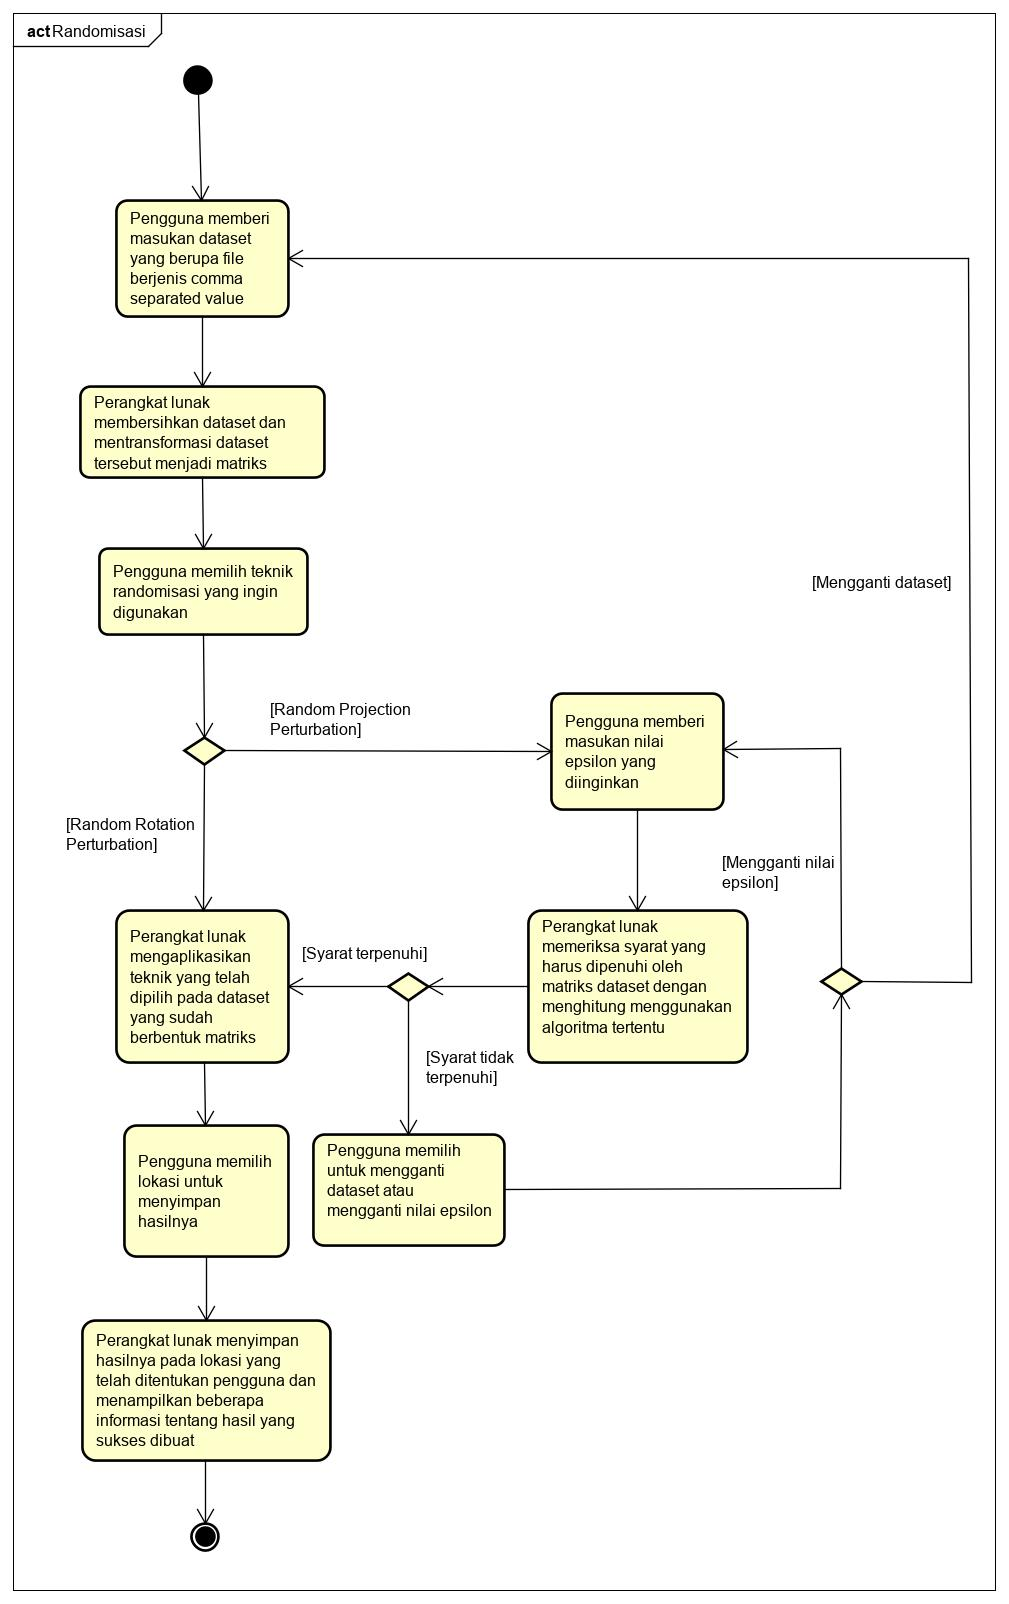
\includegraphics[scale=0.4]{activitydiagram}
    \caption{Diagram aktivitas perangkat lunak randomisasi}
    \label{fig:activitydiagram}
\end{figure}

Perangkat lunak randomisasi adalah perangkat lunak yang digunakan untuk memodifikasi data dengan metode randomisasi. Perangkat lunak ini akan memiliki fungsi untuk mengubah nilai setiap data yang dimasukan agar privasinya terjaga tetapi masih dapat dilakukan penambangan data. Algoritma \textit{Random Rotation Perturbation} dan \textit{Random Projection Perturbation} akan diimplementasikan pada perangkat lunak ini untuk fungsi utama yaitu mengubah nilai pada setiap data. Dengan mempertimbangkan studi literatur, analisis masalah, dan studi kasus yang telah dilakukan pada kedua teknik tersebut, perangkat lunak akan memiliki berbagai pilihan dan parameter yang pengguna harus masukan dan juga ada beberapa persyaratan atau batasan agar perangkat lunak ini berjalan dengan semestinya. Diagram aktivitas untuk perangkat lunak randomisasi dapat dilihat pada Gambar~\ref{fig:activitydiagram}. Detail dari diagram aktivitas tersebut adalah sebagai berikut.
\begin{enumerate}
    \item Pengguna memberikan masukan berupa dataset yang berupa file berjenis \textit{comma-separated values} (CSV). File ini harus berisi tiap rekord pada barisnya dan tiap fitur pada kolomnya. Adanya nama kolom diperbolehkan pada baris pertama dalam file tersebut
    \item Perangkat lunak akan membersihkan file yang berisi dataset tersebut dan mentransformasi datasetnya menjadi sebuah matriks. Matriks tersebut akan berisi nilai-nilai pada dataset saja tanpa nama kolom
    \item Pengguna memilih teknik randomisasi yang ingin digunakan antara \textit{Random Rotation Perturbation} dan \textit{Random Projection Perturbation}. Jika \textit{Random Projection Perturbation} yang dipiilih maka akan ada beberapa langkah yang harus dipenuhi yaitu sebagai berikut.
    \begin{enumerate}
        \item Pengguna memberi masukan nilai epsilon yang diinginkan
        \item Perangkat lunak memeriksa syarat yang harus dipenuhi oleh matriks dataset dengan menghitung menggunakan algoritma tertentu. Pengecekan ini adalah pengecekan jumlah kolom pada matriks dataset apakah cukup untuk matriks tersebut direduksi dimensinya. Jika syarat terpenuhi maka langkah selanjutnya adalah perangkat lunak mengaplikasikan teknik yang dipilih
        \item Jika syarat tidak terpenuhi maka pengguna harus memilih untuk mengganti datasetnya atau mengganti nilai epsilon
    \end{enumerate}
    \item Perangkat lunak mengaplikasikan teknik yang telah dipilih pada dataset yang sudah berbentuk matriks
    \item Pengguna memilih lokasi pada komputer pengguna untuk menyimpan hasil dari teknik yang dipilih. Hasilnya adalah sebuah file CSV yang berisi dataset yang sudah diaplikasikan teknik randomisasi
    \item Perangkat lunak menyimpan hasilnya pada lokasi yang telah ditentukan pengguna dan menampilkan beberapa informasi tentang hasil yang sukses dibuat
\end{enumerate}

\subsection{Diagram Kelas}
\label{sec:diagram-kelas}

Perancangan diagram kelas didasarkan pada analisis terhadap algoritma yang ingin diimplementasikan yaitu \textit{Random Rotation Perturbation} dan \textit{Random Projection Perturbation}, serta berdasarkan pada diagram aktivitas yang telah dibuat, dan dengan mempertimbangkan studi literatur, analisis masalah, dan studi kasus yang telah dilakukan pada kedua algoritma randomisasi yang ingin diimplementasikan. Detail dari diagram kelas perangkat lunak randomisasi pada Gambar~\ref{fig:classdiagram} adalah sebagai berikut.
\begin{itemize}
    \item Kelas \textit{Perturbation} adalah kelas abstrak yang akan di-\textit{extend} oleh kelas yang mengimplementasikan algoritma \textit{Random Rotation Perturbation} dan \textit{Random Projection Perturbation}
    \item Kelas \textit{RandomRotationPerturbation} adalah kelas yang mengimplementasikan algoritma \textit{Random Rotation Perturbation}. Kelas ini merupakan \textit{subclass} dari kelas \textit{Perturbation}
    \item Kelas \textit{RandomProjectionPerturbation} adalah kelas yang mengimplementasikan algoritma \textit{Random Projection Perturbation}. Kelas ini merupakan \textit{subclass} dari kelas \textit{Perturbation}
    \item Kelas \textit{Matrix} adalah kelas untuk merepresentasikan matriks dan menyimpan nilai-nilai pada setiap elemen matriks. Kelas ini juga memiliki fungsi perkalian yang akan digunakan untuk implementasi algoritma \textit{Random Rotation Perturbation} dan \textit{Random Projection Perturbation}
    \item Kelas \textit{RandomTranslationMatrix} adalah kelas untuk membuat matriks translasi acak. Kelas ini adalah \textit{subclass} dari kelas \textit{Matrix}
    \item Kelas \textit{RandomRotationMatrix} adalah kelas untuk membuat matriks rotasi acak. Kelas ini adalah \textit{subclass} dari kelas \textit{Matrix}
    \item Kelas \textit{RandomProjectionMatrix} adalah kelas untuk membuat matriks proyeksi acak. Kelas ini adalah \textit{subclass} dari kelas \textit{Matrix}
    \item Kelas \textit{CSVPreprocessor} adalah kelas untuk menangani masukan dataset berupa file CSV yang akan direpresentasikan menjadi matriks. Kelas ini berguna untuk mengkonversi file CSV menjadi matriks dan sebaliknya.
\end{itemize}

\begin{figure}
    \centering
    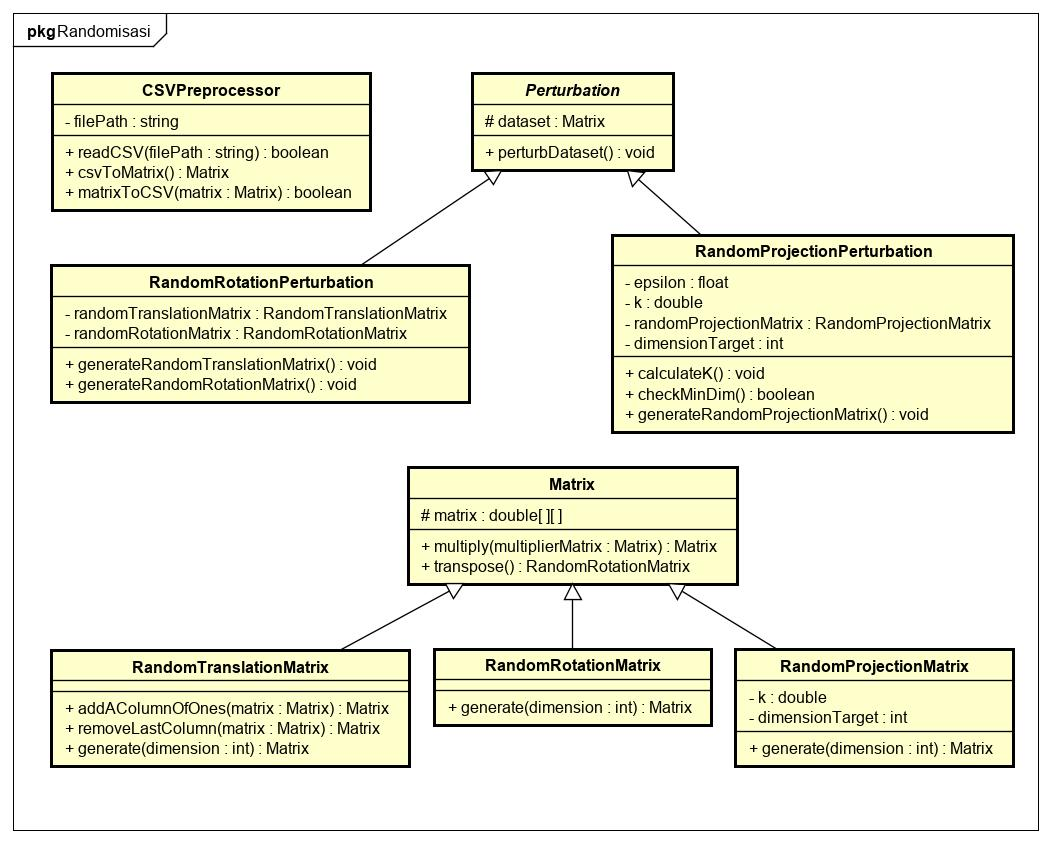
\includegraphics[scale=0.4]{classdiagram}
    \caption{Diagram kelas perangkat lunak randomisasi}
    \label{fig:classdiagram}
\end{figure}
